\documentclass{article}

\usepackage{graphicx}
\usepackage{subfigure}

\renewcommand{\figurename}{Fig.} 
\renewcommand{\thefigure}{S\arabic{figure}} 
\begin{document}

\title{Supplementary Material}
\date{}

\maketitle
%ce-hs
\begin{figure}[!htbp]
    \subfigure[CE measurement]{
        \begin{minipage}[b]{0.5\linewidth}
            \centering
            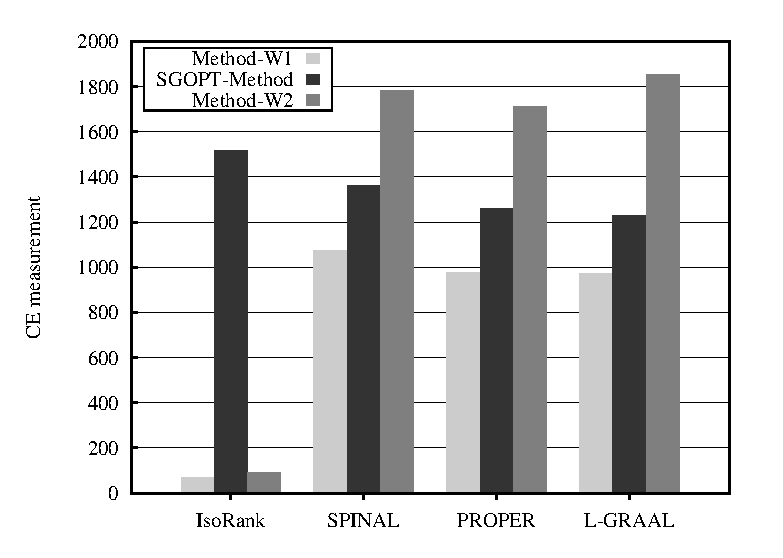
\includegraphics[width=\linewidth]{pic/ce-hs-CE.eps}
            \label{ce-hs-CE}
        \end{minipage}
    }
   \subfigure[Running Time]{
        \begin{minipage}[b]{0.5\linewidth}
            \centering
            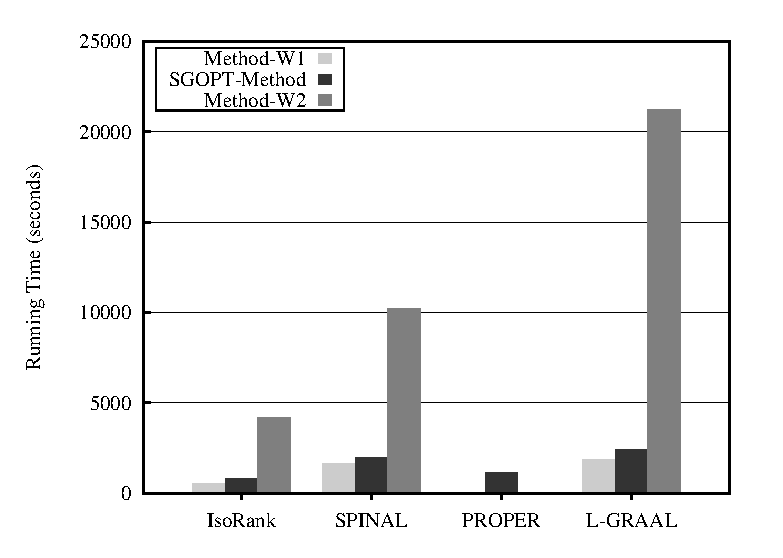
\includegraphics[width=\linewidth]{pic/ce-hs-Time.eps}
            \label{ce-hs-Time}
        \end{minipage}
    }
    \caption{Experiment results using four methods in three ways aligning C.elegans and H.sapiens PPI networks.}
    \label{ce-hs}
\end{figure}

%ce-sc
\begin{figure}[!htbp]
    \subfigure[CE measurement]{
        \begin{minipage}[b]{0.5\linewidth}
            \centering
            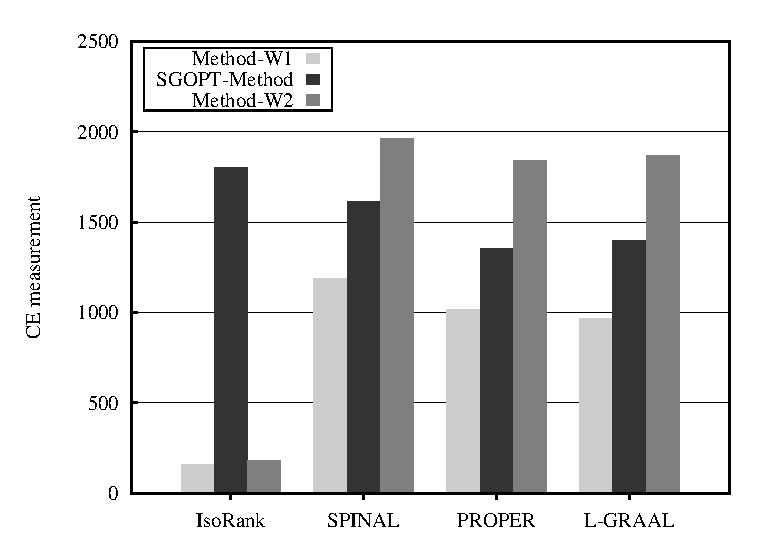
\includegraphics[width=\linewidth]{pic/ce-sc-CE.eps}
            \label{ce-sc-CE}
        \end{minipage}
    }
   \subfigure[Running Time]{
        \begin{minipage}[b]{0.5\linewidth}
            \centering
            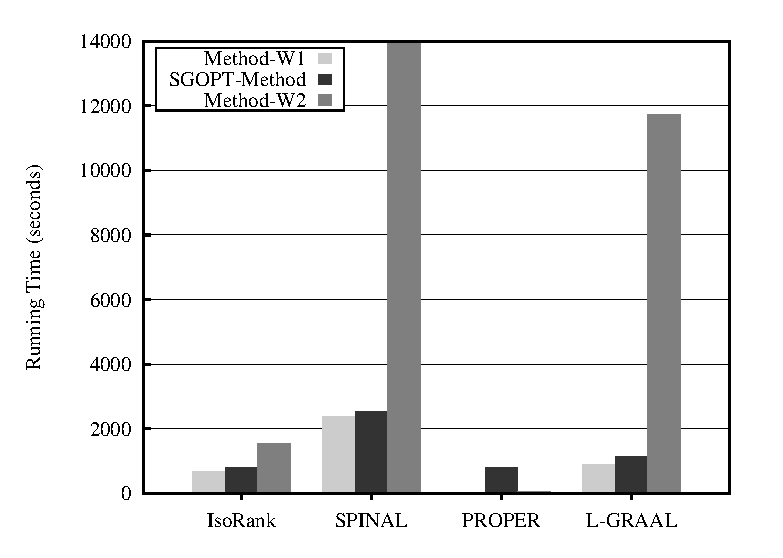
\includegraphics[width=\linewidth]{pic/ce-sc-Time.eps}
            \label{ce-sc-Time}
        \end{minipage}
    }
    \caption{Experiment results using four methods in three ways aligning C.elegans and S.cerevisiae PPI networks.}
    \label{ce-sc}
\end{figure}

%dm-hs
\begin{figure}[!htbp]
    \subfigure[CE measurement]{
        \begin{minipage}[b]{0.5\linewidth}
            \centering
            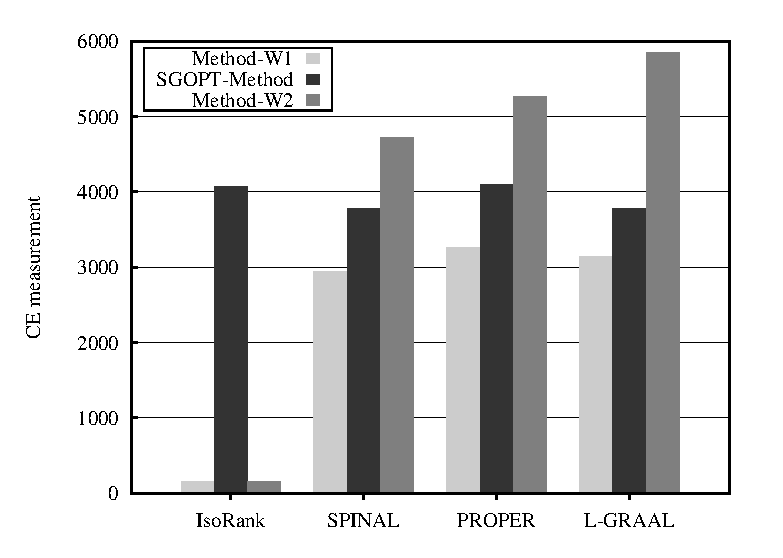
\includegraphics[width=\linewidth]{pic/dm-hs-CE.eps}
            \label{dm-hs-CE}
        \end{minipage}
    }
   \subfigure[Running Time]{
        \begin{minipage}[b]{0.5\linewidth}
            \centering
            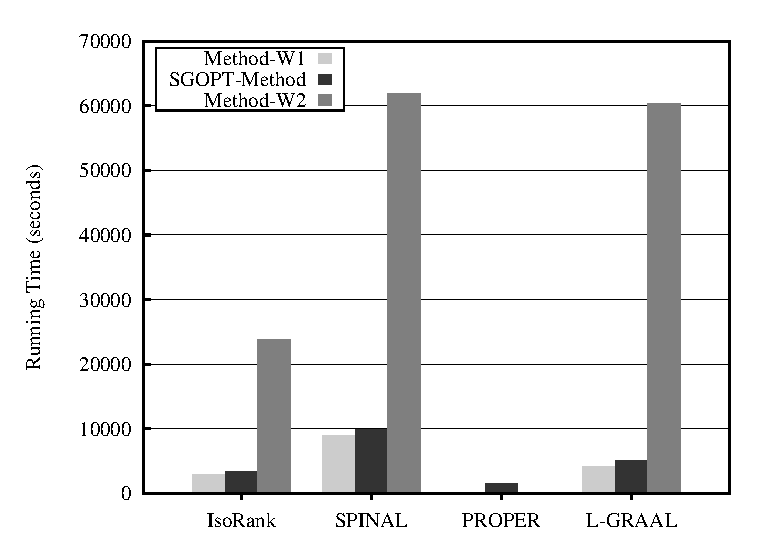
\includegraphics[width=\linewidth]{pic/dm-hs-Time.eps}
            \label{dm-hs-Time}
        \end{minipage}
    }
    \caption{Experiment results using four methods in three ways aligning D.melanogaster and H.sapiens PPI networks.}
    \label{dm-hs}
\end{figure}

%dm-sc
\begin{figure}[!htbp]
    \subfigure[CE measurement]{
        \begin{minipage}[b]{0.5\linewidth}
            \centering
            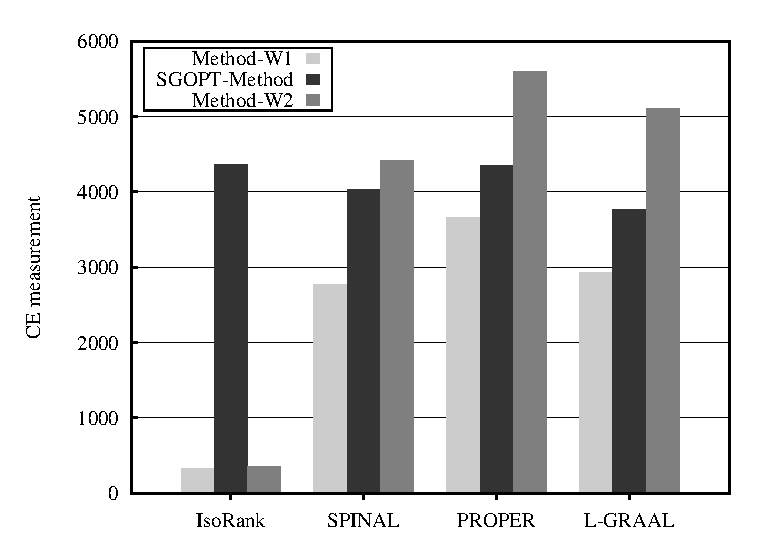
\includegraphics[width=\linewidth]{pic/dm-sc-CE.eps}
            \label{dm-sc-CE}
        \end{minipage}
    }
   \subfigure[Running Time]{
        \begin{minipage}[b]{0.5\linewidth}
            \centering
            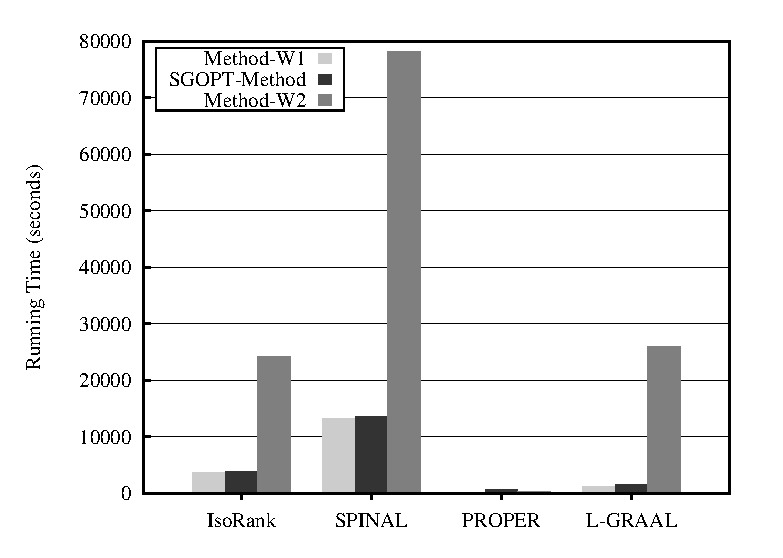
\includegraphics[width=\linewidth]{pic/dm-sc-Time.eps}
            \label{dm-sc-Time}
        \end{minipage}
    }
    \caption{Experiment results using four methods in three ways aligning D.melanogaster and S.cerevisiae PPI networks.}
    \label{dm-sc}
\end{figure}

%hs-sc
\begin{figure}[!htbp]
    \subfigure[CE measurement]{
        \begin{minipage}[b]{0.5\linewidth}
            \centering
            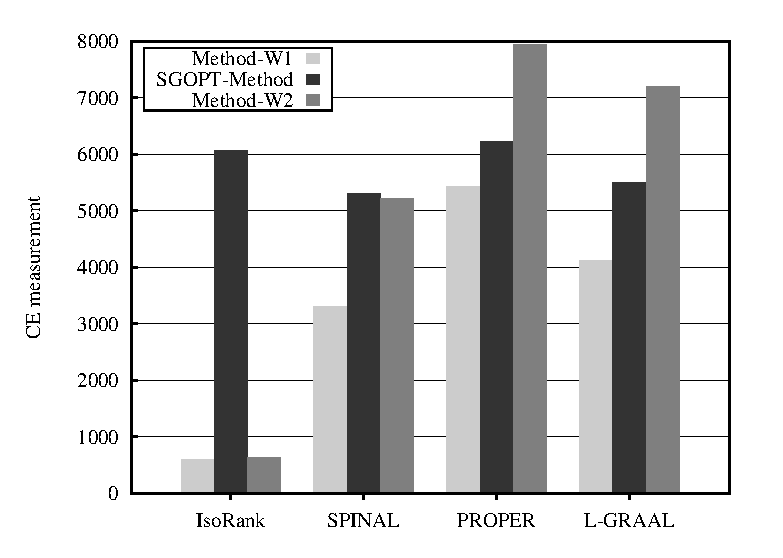
\includegraphics[width=\linewidth]{pic/hs-sc-CE.eps}
            \label{hs-sc-CE}
        \end{minipage}
    }
   \subfigure[Running Time]{
        \begin{minipage}[b]{0.5\linewidth}
            \centering
            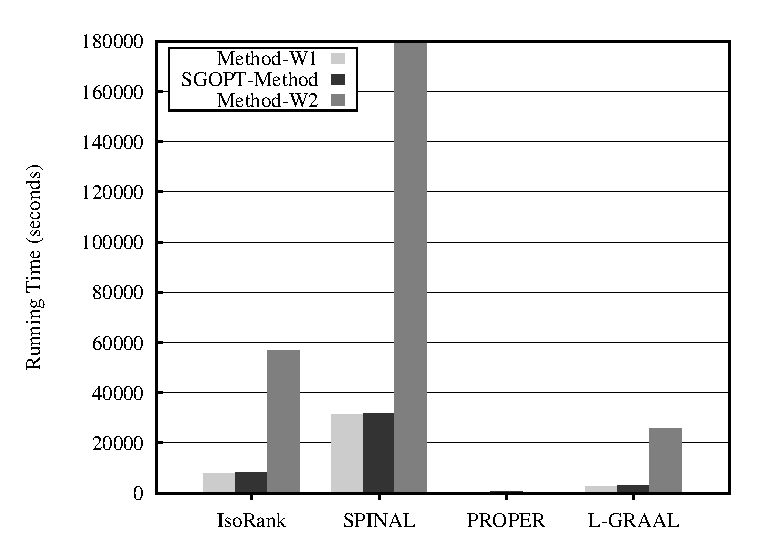
\includegraphics[width=\linewidth]{pic/hs-sc-Time.eps}
            \label{hs-sc-Time}
        \end{minipage}
    }
    \caption{Experiment results using four methods in three ways aligning H.sapiens and S.cerevisiae PPI networks.}
    \label{dm-sc}
\end{figure}


\end{document}